

In this thesis we are interested in processes involving superpartners of leptons, gauge bosons, and the Higgs boson. Besides this, we will look at a dark matter particle candidate, which is predicted by both  SUSY, to be the lightest supersymmetric particle (LSP), and by simplified non-SUSY DM models requiring a new mediator V. This thesis looks at data from proton-proton collisions at the LHC in final states of two leptons and missing transverse energy. The SUSY processes we are looking at are direct slepton production, chargino production with slepton/sneutrino-mediated-decays and with W-boson-mediated-decays. 

Figure \ref{fig:SlepSlepFeynman} shows direct slepton production with the sleptons decaying to a final state with two leptons and missing transverse energy (MET/$E_T^{miss}$ i.e. missing energy in the detector) from the lightest neutralinos ($\tilde{\chi}_1^0$). The neutralino is assumed to be stable and not measured directly by the detector. The energy of the neutralinos is therefore interpreted as MET in this process. The neutralino is a mixture of the sparticle components photino, zino, and neutral higgsino. Since it is believed to be 100\% stable  it constitutes a perfect dark matter candidate as mentioned above.  
\begin{figure}[H]
    \centering
    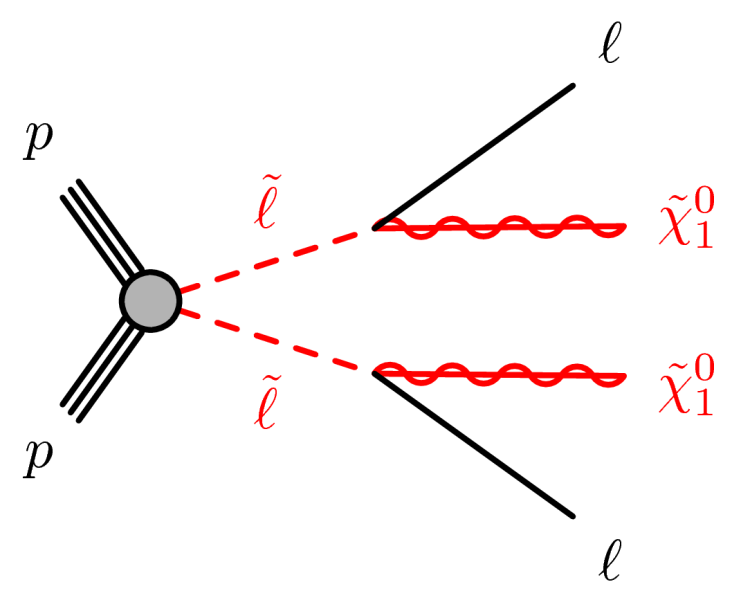
\includegraphics[width = 0.4\textwidth]{Figures/FeynmanDiagrams/SlepSlepFeynman.png}
    \caption{Direct slepton production $pp \rightarrow \tilde{l}^+ \tilde{l}^- \rightarrow l^+l^- + \tilde{\chi}_1^0 \tilde{\chi}_1^0$.}
    \label{fig:SlepSlepFeynman}
\end{figure}

In Figures \ref{fig:SlepSnuFeynman} and \ref{fig:WWFeynman} chargino production with slepton/sneutrino-mediated-decays and W-boson-mediated-decays are shown, respectively. Charginos are a mixture of the sparticle components wino and the charged higgsino. These processes have the same final state as direct slepton production, but here the neutrinos also contribute to the MET, since they connot be observed in the detector. 
\begin{figure}[H]
    \centering
    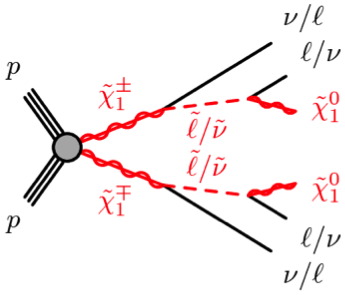
\includegraphics[width = 0.4\textwidth]{Figures/FeynmanDiagrams/SlepSnuFeynman.png}
    \caption{Chargino production with slepton/sneutrino-mediated-decays $pp \rightarrow \tilde{\chi}_1^+ \tilde{\chi}_1^- \rightarrow \tilde{l}^+ \tilde{l}^- /\tilde{\nu} \tilde{\nu} \rightarrow l^+l^- + \nu \Bar{\nu} + \tilde{\chi}_1^0 \tilde{\chi}_1^0$.}
    \label{fig:SlepSnuFeynman}
\end{figure}

\begin{figure}[H]
    \centering
    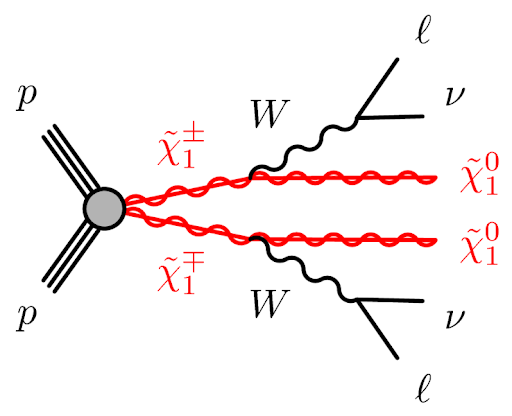
\includegraphics[width = 0.4\textwidth]{Figures/FeynmanDiagrams/WWFeynman.png}
    \caption{Chargino production with W-boson-mediated-decays $pp \rightarrow \tilde{\chi}_1^+ \tilde{\chi}_1^- \rightarrow W^+ W^- \rightarrow l^+l^- + \nu \Bar{\nu} + \tilde{\chi}_1^0 \tilde{\chi}_1^0$.}
    \label{fig:WWFeynman}
\end{figure}

The DM process we are looking at in this thesis is the mono-Z process shown in figure \ref{fig:monoZFeynman2}. Here we have a new mediator V between matter ($q\Bar{q}$) and DM (two particles $\chi$). In addition we require a Z-boson, radiated from one of the initial state particles\footnote{Initial state radiation means that one of the incoming particles emits a particle before the annihilation, e.g. the Z-boson in our process.}, which subsequently decays into two leptons. This gives us the same final state as we had for the SUSY processes above.  

\begin{figure}[H]
    \centering
    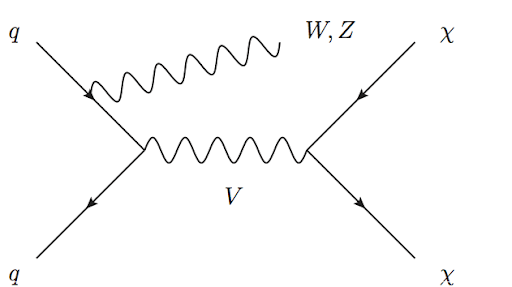
\includegraphics[width = 0.4\textwidth]{Figures/FeynmanDiagrams/monoZFeynman2.png}
    \caption{Mono-Z process $pp \rightarrow Z + MET \rightarrow l^+ l^- + MET$.}
    \label{fig:monoZFeynman2}
\end{figure}


\section{Monte Carlo simulated events}

The data considered is recorded by the ATLAS experiment at the LHC between 2015 and 2018 (Run 2), presented in chapter \ref{sec:LHCandATLAS}. But, we are also looking at MC simulated SM backgrounds and new physics signals which will be explained in this section, taken from the publications from ATLAS, namely \cite{sleptonexclusion} for the SUSY signals and \cite{monoZexclusion} for the mono-Z signal. Tables \ref{tab:directslepLOW} - \ref{tab:MonoZHigh} in section \ref{sec:sigsamptab} present an overview of the signal samples that are used. 

The SUSY signal samples were generated from leading-order (LO) matrix elements with up to two extra partons using \textsc{MadGraph5\_aMC@NLO 2.6.1} \cite{48} interfaced to \textsc{Pythia 8.186} \cite{49}, with the A14 tune \cite{50}, for the modelling of the SUSY decay chain, parton showering, hadronisation and the description of the underlying event. Parton luminosities were provided by the NNPDF2.3LO PDF set \cite{51}. Signal cross-sections were calculated to next-to-leading order (NLO) in $\alpha_s$. The nominal cross-sections and their uncertainties were taken from an envelope of cross-section predictions using different PDF sets and factorisation and renormalisation scales, as described in Ref. \cite{60}. 


The DM signal is modelled with the leading-order \textsc{MadGraph5\_aMC@NLO} matrix element \cite{54Z} using NNPDF3.0 \cite{55Z} and showered with Pythia8.186. DM signal events with an axial-vector\footnote{An axial-vector is the cross-product of two vector quantities, which will not change sign under parity transformations because both $\mathbf{v}_1$ and $\mathbf{v}_2$ do. E.g. angular momentum $\mathbf{L} = \mathbf{x} \times \mathbf{p}$, where \textbf{x} is position and \textbf{p} is momentum.} mediator and fermionic WIMPs (weakly interacting massive particles) are produced for different mediator and DM masses $m_{V}$ and $m_\chi$, both in a range from 10 to 1000 GeV.  As recommended in Ref. \cite{44Z}, the DM events are generated by choosing couplings to quarks $g_q = 0.25$, and to DM $g_\chi = 1$, and a minimal mediator width. The A14 \cite{57Z} parameter set is used to tune the \textsc{Pythia8.186} parton-shower for the simulation of the DM signal.


The different SM backgrounds we consider are diboson, triboson, $t\Bar{t}$, single top, other top events ($t\Bar{t}$ events with a pair of leptons or boson(s)), Higgs, Drell-Yan, Z+jets and W+jets. The MC samples are simulated using different generators that are listed in table \ref{tab:bkg_samples}. The goal is to separate these backgrounds from the new physics signal processes discussed earlier in the chapter. 

\begin{table}[H]
    \centering
    \begin{tabular}{l l l l} \toprule
        \textbf{Background sample} & \textbf{Generator} & \textbf{Parton shower} & \textbf{Normalisation}\\
        \midrule
        \midrule
        Diboson & \textsc{Sherpa2.2.2}\cite{sherpa2_1, sherpa1_2, sherpa1_3} & \textsc{Sherpa2.2.2} & NLO \cite{NLO}\\
        Triboson & \textsc{Sherpa2.2.2} & \textsc{Sherpa2.2.2} & NLO \\
        Z+jets & \textsc{Sherpa2.2.1} \cite{sherpa1_1, sherpa1_2, sherpa1_3} & \textsc{Sherpa2.2.1} & NNLO \cite{NNLO}\\
        W+jets & \textsc{Powheg-Box v2}\cite{49Z, 50Z} & \textsc{Pythia8.186} \cite{49} & NLO\\
        Drell-Yan & \textsc{Sherpa2.2.1} & \textsc{Sherpa2.2.1} & NNLO\\
        $t\Bar{t}$ & \textsc{Powheg-Box v2} & \textsc{Pythia8.186} & NNLO\\
        Single top & \textsc{Powheg-Box v2} & \textsc{Pythia8.186} & NLO\\
        topOther & \textsc{MG5\_aMC@NLO} \cite{48} & \textsc{Pythia8.186} & NLO\\
        Higgs & \textsc{Powheg-Box v2} & \textsc{Pyhtia8.186} & NLO\\
        \bottomrule
    \end{tabular}
    \caption{An overview of the different generators used to simulate the MC background samples.}
    \label{tab:bkg_samples}
\end{table}

Before we move to the analysis searching for SUSY and DM signals exploiting machine learning techniques we need to make sure that our input (i.e data, SM background and new physics signal MC) looks reasonable. We also need a baseline analysis to check whether or not the ML analysis perform better than the more standard cut and count analysis, which will be outlined in the following sections.


\begin{comment}

Before we move to how we perform the analysis, we also need to know how we are going to know that we see SUSY and DM particles in the detector. Since they never have been discovered, we have to lean on some hypotheses on how this is happening. As for all events in the detector, we have to reconstruct the events using their decays. The supersymmetric particles are expected to decay into cascades that will contain an LSP which will interact very weakly with the detector material which again will result in large MET in the detector. The rest of the cascade will result in a final state with leptons and/or jets. Together with MET this gives us the final state we are looking for. For the mono-Z process we can measure the MET from the DM particles decayed from the unknown hypothetical mediator particle. Together with the leptons we get from the decay of the Z-boson, this gives us the same final state as for the SUSY processes.


\end{comment}


































\begin{comment}

\begin{itemize}
    \item Bruker noe som eksisterer
    \item Tradisjonell måte ting har blitt gjort på
    \item begrenset av menneskets forståelse av prosessen vi ser på
    \item vi må bestemme alle kuttene som blir gjort
    \item Du må vite hva du skal se etter for å gjøre dette, altså trenger en teori/hypotese
    \item Tenk overgang til ML
    \item Valg må være begrunnet 
    \item Massesplitting. Cut and count er svak på lav massesplitting. Dette gjør ML bedre
\end{itemize}
\end{comment}





